\subsection{Konzept und Idee}

Die Idee ist es, ein SmartHome zu entwickeln, welches auf einem 8051 Microcontroller als Grundlage aufbaut. Dabei sollen drei Hauptfunktionen eines modernen SmartHomes über diesen gesteuert werden.

\subsubsection{Heizung}
Die erste Funktion ist eine Temperatursteuerung für die Fußbodenheizung. Dabei soll die Fußbodenheizung in einem Haus so gesteuert werden, dass diese automatisch eingeschaltet wird, sobald die Temperatur unter einen festen Wert fällt. Außerdem soll der Nutzer mit Hilfe eines Schalters festlegen können, ob die Heizung dauerhaft an oder in einen automatischen Modus eingestellt ist. Der Temperatursensor ist zusätzlich abschaltbar, damit die Heizung ausgeschaltet werden kann.

Wird der Heizungsschalter auf An gestellt, läuft die Heizung unabhängig von der Temperatur die ganze Zeit. Wird dieser auf den Automodus gestellt, kommt es auf den Temperatursensor an, da dieser unabhängig von der Heizung ein bzw. ausgeschaltet werden kann. Ist dieser eingeschaltet, schaltet sich die Heizung an, sobald die Temperatur unter einen bestimmten Wert fällt.
Aus diesen Anforderungen ergibt sich eine Tabelle aus der alle möglichen Eingaben und Ausgabemöglichkeiten ausgelesen werden können. Aus diesen geht ein Schaltplan hervor, welcher für die Programmierung des 8051 Microcontrollers genutzt wird.
Die Tabelle sieht wie folgt aus:

\begin{table}[htbp]
\centering
\caption{Schaltplan Heizungssteuerung}
\label{my-label}
\begin{tabular}{|l|l|l|l|}
\hline
\multicolumn{1}{|c|}{\textbf{Heizungsschalter}} & \multicolumn{1}{c|}{\textbf{Temperatursensor Schalter}} & \multicolumn{1}{c|}{\textbf{Temperatur < Wert}} & \multicolumn{1}{c|}{\textbf{Heizung An?}} \\ \hline
 0 & 0 & 0 & 0 \\ \hline
 0 & 0 & 1 & 0 \\ \hline
 0 & 1 & 0 & 0 \\ \hline
 0 & 1 & 1 & 1 \\ \hline
 1 & 0 & 0 & 1 \\ \hline
 1 & 0 & 1 & 1 \\ \hline
 1 & 1 & 0 & 1 \\ \hline
 1 & 1 & 1 & 1 \\ \hline
\end{tabular}
\end{table}

Für diese Steuerung wird die Schaltung nach diesem Schaltplan programmiert:

\begin{figure}[htbp] 
  \centering
     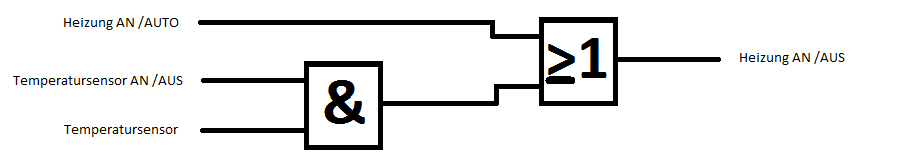
\includegraphics[width=0.7\textwidth]{Heizungsschaltung.png}
  \caption{Schaltung für die Heizung}
  \label{fig:Bild1}
\end{figure}

Dabei kommen die Eingaben aus dem Port 2.0 bis 2.2 und die Ausgabe ist auf dem Port 3.4.

\subsubsection{Licht}
Die zweite Funktion ist eine Lichtsteuerung für das Licht. Der Nutzer soll die Möglichkeit haben das Licht mit Hilfe eines Bewegungssensors ein beziehungsweise aus zu schalten. Dieser Sensor ist zusätzlich an einen Schalter angeschlossen, um diesen An bzw. Aus zu schalten.
 
Aus diesen Anforderungen ergibt sich eine Tabelle aus der alle möglichen Eingaben und Ausgabemöglichkeiten ausgelesen werden können. Aus diesen geht ein Schaltplan hervor, welcher für die Programmierung des 8051 genutzt wird.

\begin{table}[htbp]
\centering
\caption{Schaltplan Lichtsteuerung}
\label{my-label}
\begin{tabular}{|l|l|l|}
\hline
\multicolumn{1}{|c|}{\textbf{Bewegungssensor}} & \multicolumn{1}{c|}{\textbf{Schalter}} & \multicolumn{1}{c|}{\textbf{Licht an?}} \\ \hline
 0 & 0 & 0 \\ \hline
 0 & 1 & 0 \\ \hline
 1 & 0 & 0 \\ \hline
 1 & 1 & 1 \\ \hline
\end{tabular}
\end{table}

Für diese Steuerung wird die Schaltung nach diesem Schaltplan programmiert:

\begin{figure}[htbp] 
  \centering
     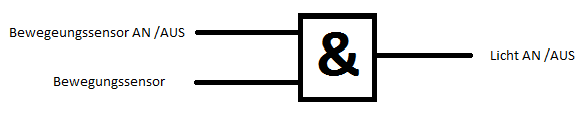
\includegraphics[width=0.7\textwidth]{Lichtschaltung.png}
  \caption{Schaltung für das Licht}
  \label{fig:Bild2}
\end{figure}

Dabei kommen die Eingaben aus den Ports P1.0 und 1.1 und die Ausgabe ist auf dem Port 3.5.

\subsubsection{Rollläden}
Der dritte Teil der SmartHome Steuerung ist eine Steuerung für Rollläden. Diese werden in zwei Modi betrieben. Im automatischen Modus sollen sie sich automatisch öffnen, sobald es draußen hell, beziehungsweise schließen, sobald es draußen dunkel wird. Es wird ein Helligkeitssensor benötigt, der ein bit setzt, sobald es hell ist und umgekehrt. Der zweite Modus ist eine manuelle Steuerung. Für jeden Rollladen gibt es je zwei Schalter, die für Rollladen Hoch, beziehungsweise für Rollladen runter, stehen. Beide Modi werden durch Sensoren unterstützt, die jeweils anzeigen, ob ein Rollladen geschlossen oder ganz geöffnet ist. 
Aus diesen Anforderungen gehen wie zuvor auch diese Tabellen für die beiden Modi hervor:

\begin{table}[]
\centering
\caption{Rolladensteuerung manuell}
\label{my-label}
\begin{tabular}{|l|l|l|l|l|l|}
\hline
\multicolumn{1}{|c|}{\textbf{SR Oben}} & \multicolumn{1}{c|}{\textbf{SR Unten}} & \multicolumn{1}{c|}{\textbf{SR Hoch}} & \multicolumn{1}{c|}{\textbf{SR Runter}} & \multicolumn{1}{c|}{\textbf{MR Hoch}} & \multicolumn{1}{c|}{\textbf{MR Runter}} \\ \hline
 0 & 0 & 0 & 0 & 0 & 0 \\ \hline
 0 & 0 & 0 & 1 & 0 & 1 \\ \hline
 0 & 0 & 1 & 0 & 1 & 0 \\ \hline
 0 & 0 & 1 & 1 & 0 & 0 \\ \hline
 0 & 1 & 0 & 0 & 0 & 0 \\ \hline
 0 & 1 & 0 & 1 & 0 & 0 \\ \hline
 0 & 1 & 1 & 0 & 1 & 0 \\ \hline
 0 & 1 & 1 & 1 & 0 & 0 \\ \hline
 1 & 0 & 0 & 0 & 0 & 0 \\ \hline
 1 & 0 & 0 & 1 & 0 & 1 \\ \hline
 1 & 0 & 1 & 0 & 0 & 0 \\ \hline
 1 & 0 & 1 & 1 & 0 & 0 \\ \hline
 1 & 1 & 0 & 0 & 0 & 0 \\ \hline
 1 & 1 & 0 & 1 & 0 & 0 \\ \hline
 1 & 1 & 1 & 0 & 0 & 0 \\ \hline
 1 & 1 & 1 & 1 & 0 & 0 \\ \hline
\end{tabular}
\end{table}


\begin{table}[]
\centering
\caption{Rolladensteuerung automatisch}
\label{my-label}
\begin{tabular}{|l|l|l|l|l|}
\hline
\multicolumn{1}{|c|}{\textbf{SR Oben}} & \multicolumn{1}{c|}{\textbf{SR Unten}} & \multicolumn{1}{c|}{\textbf{Helligkeitssensor}} & \multicolumn{1}{c|}{\textbf{MR Hoch}} & \multicolumn{1}{c|}{\textbf{MR Runter}} \\ \hline
0 & 0 & 0 & 0 & 1 \\ \hline
0 & 0 & 1 & 1 & 0 \\ \hline
0 & 1 & 0 & 0 & 0 \\ \hline
0 & 1 & 1 & 1 & 0 \\ \hline
1 & 0 & 0 & 0 & 1 \\ \hline
1 & 0 & 1 & 0 & 0 \\ \hline
1 & 1 & 0 & 0 & 0 \\ \hline
1 & 1 & 1 & 0 & 0 \\ \hline
\end{tabular}
\end{table}
Die Signale aus Sensoren und Schalter sollen über P0, sowie über P2.6 und P2.7 eingegeben werden. Die Ausgabe an die Motoren erfolgt über P3.0 - P3.3
